\documentclass[12pt,a4paper]{article}
\usepackage[utf8]{inputenc}
\usepackage{amsmath}
\usepackage{amsfonts}
\usepackage{amssymb}
\usepackage{graphicx}
\usepackage{geometry}
\usepackage{doclicense}

%\usepackage[backend=bibtex,style=authoryear,natbib=true]{biblatex} % Use the bibtex backend with the authoryear citation style (which resembles APA)
\usepackage[backend=bibtex,style=numeric,natbib=true]{biblatex} % Use the bibtex backend with the authoryear citation style (which resembles APA)

\addbibresource{bibliograph.bib} % The filename of the bibliography

\usepackage[autostyle=true]{csquotes} % Required to generate language-dependent quotes in the bibliography

\usepackage{listings}
\usepackage{color}
\definecolor{purple}{rgb}{0.502,0,0.502}
\definecolor{amethyst}{rgb}{0.6,0.4,0.8}
\definecolor{blue}{rgb}{0,0,0.8}
\definecolor{black}{rgb}{1,1,1}
\definecolor{lightgray}{gray}{0.3}
\definecolor{gray}{gray}{0.6}
\definecolor{backcolour}{rgb}{0.95,0.95,0.92}
\renewcommand{\lstlistingname}{Code}
\lstdefinestyle{hdl}	{
    language=vhdl,
    backgroundcolor=\color{backcolour},
    commentstyle=\color{lightgray},
    keywordstyle=\color{purple},
    numberstyle=\tiny\color{gray},
    stringstyle=\color{blue},
    basicstyle=\footnotesize,
    breakatwhitespace=false,
    xleftmargin=\parindent,
    frame=L,
    breaklines=true,
    captionpos=b,
    keepspaces=true,
    numbers=left,
    numbersep=10pt,
    showspaces=false,
    showstringspaces=false,
    showtabs=false,
    tabsize=2
}
\lstdefinestyle{shell}	{
    language=sh,
    backgroundcolor=\color{backcolour},
    commentstyle=\color{lightgray},
    keywordstyle=\color{amethyst},
    numberstyle=\small\color{gray},
    stringstyle=\color{blue},
    basicstyle=\footnotesize,
    breakatwhitespace=false,
    xleftmargin=\parindent,
    frame=L,
    breaklines=true,
    captionpos=b,
    keepspaces=true,
    numbers=left,
    numbersep=10pt,
    showspaces=false,
    showstringspaces=false,
    showtabs=false,
    tabsize=2
}
\lstdefinestyle{c}	{
    language=c,
    backgroundcolor=\color{backcolour},
    commentstyle=\color{lightgray},
    keywordstyle=\color{amethyst},
    numberstyle=\small\color{gray},
    stringstyle=\color{blue},
    basicstyle=\footnotesize,
    breakatwhitespace=false,
    xleftmargin=\parindent,
    frame=L,
    breaklines=true,
    captionpos=b,
    keepspaces=true,
    numbers=left,
    numbersep=10pt,
    showspaces=false,
    showstringspaces=false,
    showtabs=false,
    tabsize=2
}

\geometry{
    paper=a4paper, % Change to letterpaper for US letter
    inner=2.0cm, %2.5cm, % Inner margin
    outer=2.0cm, %3.8cm, % Outer margin
    bindingoffset=.5cm, % Binding offset
    top=1.5cm, % Top margin
    bottom=1.5cm, % Bottom margin
    %showframe, % Uncomment to show how the type block is set on the page
}

\author{Alexander Zoellner}
\title{Tutorial for Hardware Interrupts with the Xilinx Zynq Platform Using Linux}

\begin{document}

\maketitle
\begin{figure}[b]
    \centering
    \doclicenseThis
\end{figure}


\newpage

\tableofcontents

\newpage

\section{Introduction}
Interrupts are an essential part for communication between hardware and software.
Using interrupts prevents wasting precious CPU clock cycles on polling as well as improving the systems' responsiveness.

The Xilinx Zynq 7000 system-on-chip (SoC) series offers a number of interrupt ports between programmable logic (PL) - the FPGA side - and the processing system (PS) - the CPU.
This requires a logic implementation on the FPGA side, which can be either one of the interrupt capable IP cores of Xilinx or a custom logic.
On the CPU(s), software for configuring and receiving interrupts has to be executed.
This software can be run bare-metal (without an operating system) or with an operating system such as Linux.
The former is well covered by online tutorials and is pretty straight forward to get a working system.
Accomplishing the same using Linux, however, is not that well covered despite being an integral part even when using trivial logic such as timers.
\newline

Since it required quite some effort collecting information from user manuals, forum posts and online documentation in order to get interrupts to work with Linux, I would like to spare others (and myself in the future) the trouble of having to repeat the same all over.
\newline

%This guide is split into two sections.
Section~\ref{quick} is for the impatient and those who just want to get the job done without caring too much about the details.
Therefore, presented information are kept to a minimum and as generally applicable to other systems as possible.
A basic understanding of the work flow with Xilinx's Vivado, compiling a Linux image for a particular board and basic understanding of Linux device drivers are required.

%The second part of this guide, Section~\ref{example}, is for those who want a more detailed explanation (or are new to the Zynq platform or Linux device drivers).
%A basic example system is provided which demonstrates generating interrupt events using a timer in programmable logic and a device driver for processing the interrupt events.

\section{Quick Solution}\label{quick}
Getting PL interrupts to work in Linux requires a number of steps which can be
summarized as following.

\begin{itemize}
    \item Enable PL-PS interrupt ports in the Processing System in Vivado
    \item Connecting a port of an IP core to the enabled port
    \item Adding a devicetree entry
    \item Registering the interrupt in the device driver
\end{itemize}


Code~\ref{code:devicetree-binding} shows the entry for the devicetree for the device using the interrupt.
The first line is the name of the node which can be chosen arbitrarily as long as it does not conflict one of the existing nodes.
The second line (\emph{interrupt-parent}) references the \emph{phandle} of the interrupt handler of the system.
The value between the braces has to match the one of the interrupt handlers phandle.
The example shows the value \emph{0x4} since the devicetree binary (.dtb) has been decompiled back to the devicetree source (.dts) where all strings have been replaced by actual numbers.

The last line (\emph{interrupts}) defines the actual interrupt to be used.
In case of the general interrupt control of arm (which is used by the Zynq platform) interrupts are defined using three cells.
The first cell is always set to zero (0) for PL interrupts (see Section~\ref{kernel}).

The second cell is the interrupt number, which is the interrupt id of the PS which the PL connects to minus 32.
The Zynq platform offers a total of 16 interrupt ports with interrupt ids 91 to 84 and from 68 to 61.
The ports are connected lowest (0) to highest index (15) to the interrupt ids in the same manner, i.e. 61 to 91.
Thus, port 0 connects to interrupt id 61, which in turn results in the interrupt number 29 (61 - 32).

The last cell is used for defining the type and level of the interrupt, i.e. the condition which have to be met for an interrupt to occur.
For PL interrupts the cell can either have the value 1 or 4.
The former is \emph{low-to-high edge triggered} and the latter \emph{active high level-sensitive}.
In most cases 1 is what you want for interrupts.

SPI (shared processor interrupts), interrupt number, type and level
\lstset{style=c, caption={Devicetree entry}}
\begin{lstlisting}[label=code:devicetree-binding]
    hw_timer_0 {
        interrupt-parent = <0x4>;
        interrupts = <0 29 1;
    }
\end{lstlisting}

After compiling the devicetree source back to the devicetree binary the interrupt has to be registered by the device driver.

Code~\ref{code:req-irq} shows a minimal example for requesting the interrupt number and registering an interrupt handler.
The first two lines are the required header files which have to be included for devicetree related function calls.
The lower part after (...) can be placed in either the \emph{init} or \emph{open} (prefered) function.
The second argument of \emph{of\_find\_node\_by\_name} has to match the name used in the devicetree entry.
Subsequently, the node is passed to \emph{irq\_of\_parse\_and\_map} for registering the interrupt number.
The return value is the index of the interrupt which gets displayed in the first column when calling \emph{cat /proc/interrupts}.
Lastly, \emph{request\_irg} installs the interrupt handler which gets called when an interrupt occurs.

\lstset{style=c, caption={Device driver entry}}
\begin{lstlisting}[label=code:req-irq]
    #include <linux/of_irq.h>
    #include <linux/of.h>

        (...)

    struct device_node *np;

    np = of_find_node_by_name(NULL, "hw_timer_0");
    timer_irq = irq_of_parse_and_map(np, 0);
    request_irq(timer_irq, &timer_intr_handler, 0, "hw_timer_intr", NULL);
\end{lstlisting}

Please make sure that the hardware (PL) does not generate any interrupt events prior to successfully registering the interrupt.
\section{Hardware Timer Example}

\subsection{Introduction}\label{demo-intro}
This section describes the demonstrator system which uses a timer in programmable logic for generating interrupts on the Xilinx Zynq platform.


\subsection{Prerequisites}
The demonstrator system has been implemented on the Digilent Zybo Z7-20 board with Xilinx Vivado 2018-3.
If you want to use the demonstrator system directly, the aforementioned board is required with a Vivado installation containing the board support package.
Any Vivado installation \emph{should} work.
If you use a Zybo Z7 board, a Vivado version 2018.x and later is more convenient since you will not have to backport devicetrees and menuconfig when building the Linux image.
See Appendix~\ref{Vivado-bitstream} if you want to use a different board or are interested in how to manually build the system on the FPGA for generating the bitstream.

Debian 9 with Linux kernel 4.19 is used as the Linux image on the Zybo board, which boots from a micro SD card.
The image has been built using this \cite{DebianImage} guide.
See Appendix~\ref{Linux-Image} for details regarding the Linux image.

The prerequisites can be summarized as follows:
\begin{itemize}
\item Vivado installation (version 2017.x and later /emph{should} work)
\item A evaluation board with a Zynq 7000 chip (e.g. ZedBoard, MicroZed, Zybo, Zybo Z7)
\item Board support package for the board to be used in Vivado
\end{itemize}

\subsection{Hardware Implementation}


\subsection{Linux Kernel}\label{kernel}
%"Documentation/devicetree/bindings/interrupt-controller/arm,gic.yaml"

%kernel version: 4.19
% commit on linux-xlnx: 0ee2ead168af335315b6cd8c55cbf6e45998f585
% commit on u-boot-xlnx: 195c620e348891ca2d90c759781413f2adb3f748

\subsection{Linux User Space}

\subsubsection{Generating Interrupts}

The user space application for using the kernel module is pretty straight forward.
It can be compiled using the provided Makefile on either the host platform (using the Xilinx cross-compile tool-chain) or directly on the target.
The Xilinx environment has to be sourced first for cross compiling.
Otherwise, just copy the Makefile and timer.c file on the target (e.g. Zybo Z7 board) or use a different method such as \emph{sshfs} to mount a directory of your host on the target.

The kernel module can be compiled in the same way as the user program.

As a first step, load the kernel module as shown in figure~\ref{fig:enable-logic}.
The output of \emph{dmesg} should show that the kernel module has been loaded successfully.

\begin{figure}[ht]
    \centering
    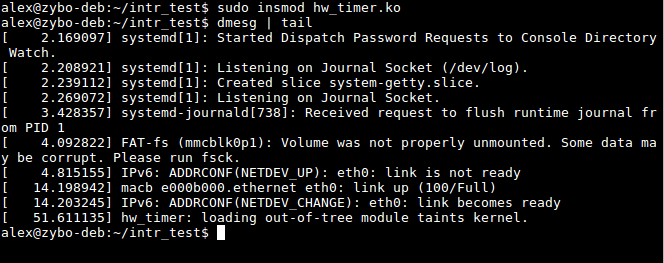
\includegraphics[width=1.0\textwidth,height=1.0\textheight,keepaspectratio]{figures/loaded_driver.png}
    \caption{Loading the kernel module}
    \label{fig:enable-logic}
\end{figure}

Figure~\ref{interrupt-list} shows the available interrupts for all CPUs.
The interrupt for our timer has been registered with number 45 in the list.
The actual interrupt number is displayed as 61 and is triggered on a (positive) edge.
The zeroes at the CPU columns indicate that no interrupt has been generated yet.

\begin{figure}[ht]
    \centering
    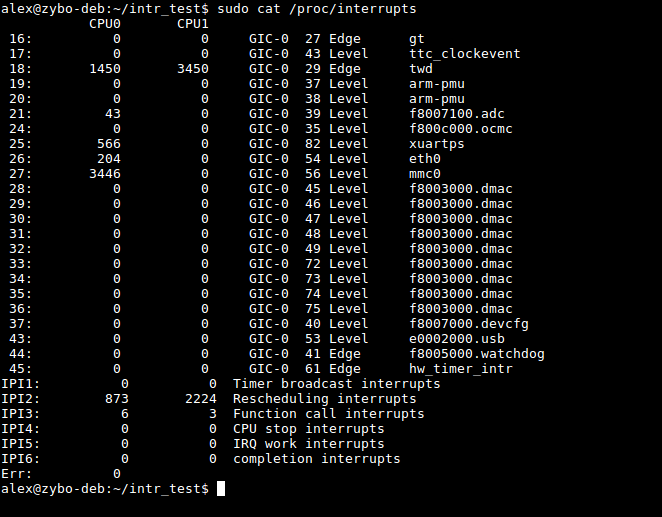
\includegraphics[width=1.0\textwidth,height=1.0\textheight,keepaspectratio]{figures/interrupt_entry.png}
    \caption{List of interrupts before generating timer interrupts}
    \label{fig:interrupt-list}
\end{figure}

Executing the test program compiled from timer.c gives the output shown in figure~\ref{fig:user-program}.

\begin{figure}[ht]
    \centering
    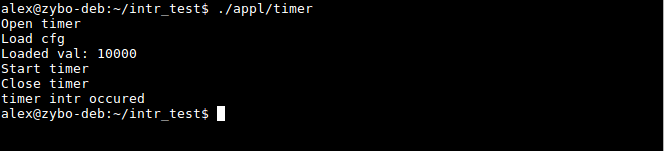
\includegraphics[width=1.0\textwidth,height=1.0\textheight,keepaspectratio]{figures/execute_user.png}
    \caption{Output of user program interfacing the kerne module}
    \label{fig:user-program}
\end{figure}

Looking at the list of interrupts again should now display a one for the column of CPU0 as shown in figure~\ref{fig:generated-interrupt}.

\begin{figure}[ht]
    \centering
    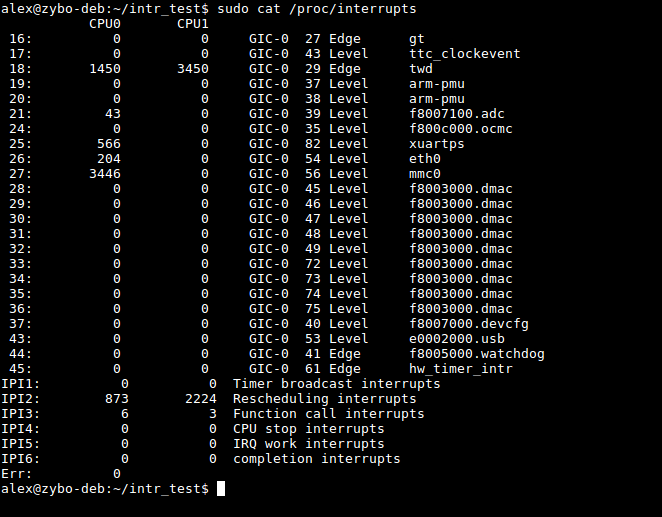
\includegraphics[width=1.0\textwidth,height=1.0\textheight,keepaspectratio]{figures/interrupt_entry.png}
    \caption{List of interrupts before generating timer interrupts}
    \label{fig:generated-interrupt}
\end{figure}

\subsubsection{Access Permissions}
It may be necessary to execute the user program with privileged access righs (using sudo).
If the device added by the kernel module should also be accessible by other users, a udev rule can be added to change permissions automatically when the device is added to the file system.
Figure~\ref{fig:udev-rule} shows the content of the rule and its path on the file system.
Just create a new file containing the shown content.

\begin{figure}[ht]
    \centering
    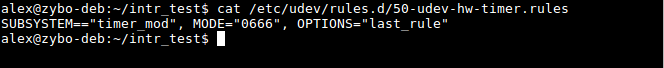
\includegraphics[width=1.0\textwidth,height=1.0\textheight,keepaspectratio]{figures/udev_rule.png}
    \caption{Changing device permissions}
    \label{fig:udev-rule}
\end{figure}

The udev rule should change permissions to the \emph{/dev/timer\_dev} as shown in figure~\ref{fig:file-permission}.

\begin{figure}[ht]
    \centering
    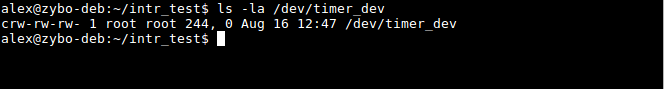
\includegraphics[width=1.0\textwidth,height=1.0\textheight,keepaspectratio]{figures/device_permission.png}
    \caption{Device permission after adding udev rule}
    \label{fig:file-permission}
\end{figure}

Figure~\ref{fig:device-info} shows how obtain the \emph{SUBSYSTEM} of the kernel module in case you want to add a similar udev rules for other devices.
\begin{figure}[ht]
    \centering
    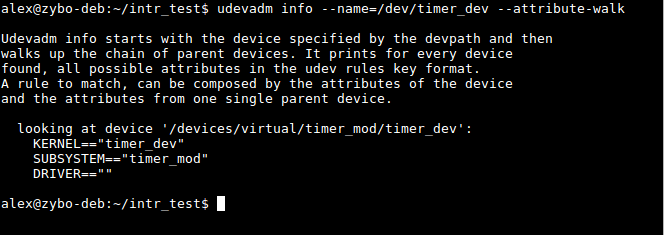
\includegraphics[width=1.0\textwidth,height=1.0\textheight,keepaspectratio]{figures/device_info.png}
    \caption{Getting detailed information for target device}
    \label{fig:device-info}
\end{figure}


\printbibliography[heading=bibintoc]


\end{document}
